\chapter{Compact Representation} \label{chapter: Compact Representation}
\section{Introduction}
Programming languages weren't designed to be presented on small screens, and therefore when you try to present programs on small screens it is difficult to read them. Programming languages are textual, and so require a keyboard In order to edit programs. Standard on-screen keyboards are inconvenient for texting, let alone for programming. In addition, they require one third of the screen which makes the small screen even smaller. Our approach is to use conventional languages such as Java and C++, but allow each programmer to have a tailored compact view that fits a small screen. We believe that we should support programmers better in doing what they already know how to do instead of requiring them to learn a new language and tools only for the purpose of sometimes developing code on mobile phones. Deverywhere is not a new language; it is a way for each programmer to see the code in the way that makes the most sense to him or her. Our solution for small screens is a compact representation of the code, which means focusing on the important information necessary to understand the code. 

This chapter discusses how the code can be presented in compact representation. It covers most of the major domains of programming idioms. Every topic that discussed in this chapter is accompanied with an explanation how it will be configurable by the user and examples of is provided by default.
\section{Operators}
This section discusses how atomic operators will be represented. Every symbol may be modified by the user to any character or icon that s/he wants.
\subsection{Basic Operators}
\autoref{tab12} provides a set of basic atomic operators that used in almost every line of code.

\begin{table}[H]
\centering
\begin{tabular}{|l|l|}
\hline
{\bf Operator} & {\bf Symbol} \\ \hline
Plus & + \\ \hline
Minus & - \\ \hline
Multiplication & * \\ \hline
Division & / \\ \hline
Modulo & \% \\ \hline
Increment & ++ \\ \hline
Decrement & - - \\ \hline
Null & $ \perp $ \\ \hline
Shift & $ \ll $; $ \gg $; $ \ggg $ \\ \hline
Relational & <; >; $ \leq $; $ \geq $ \\ \hline
Equality & =; $ \neq $ \\ \hline
Bitwise AND & \& \\ \hline
Bitwise exclusive OR & $ \textasciicircum $ \\ \hline
Bitwise inclusive OR & | \\ \hline
Logical AND & $ \wedge $  \\ \hline
Logical OR & $ \vee $  \\ \hline
Ternary & ?; : \\ \hline
Assignment & $ \longleftarrow $; +$ \longleftarrow $; -$ \longleftarrow $; *$ \longleftarrow $; /$ \longleftarrow $; \%$ \longleftarrow $; \&$ \longleftarrow $; $ \wedge $$ \longleftarrow $; $ \vee $$ \longleftarrow $; $ \ll $$ \longleftarrow $; $ \gg $$ \longleftarrow $; $ \ggg $$ \longleftarrow $\\ \hline
\end{tabular}
\caption{This table presents operators and symbols that represent them in compact representation. The symbols are examples for how symbols may be presented. The user may modify to any representation that s/he wants. This idea is discussed in \autoref{chapter:Configuration of Representation}. Note: ; is used as a separator between operator symbols.}
\label{tab12}
\end{table}
\section{Statement Terminators}
A statement terminator is used to demarcate the end of an individual statement. For example, a statement terminator in Java is ';' (semicolon) similarly to C, C++ and other programming languages. This character doesn't gives any information except where the statement end. The programmer will be able to modify the symbol, s/he may decide if it will be displayed or how will it looks like, e.g., result $ \longleftarrow $ nextNode.data, this is a line of code that missing statement terminator symbol. It is also possible to modify the style of the terminators or to use an icon.
\section{Mathematical Expressions}
Mathematical expressions are very common in programming. Sometimes they can be very long and complex. Therefore, we would like to represent those expressions in more compact and native way. We can reduce expressions length by changing mathematical expressions representation to native mathematical representation, e.g., $ (a-b)/(c-d) \longleftarrow \frac{a-b}{c-d} $.
\section{Boolean expressions}
This section discuses compact representation of boolean expressions.
\subsection{Range} \label{subsection: Range}
In-order to check if an integer is in a range the programmer needs write to write $ 0 <= i \&\& i < 10 $. We propose to write this expression in a natural representation, it will save space and will be easier for reading. For example, $ 0 \leq i < 10 $.
\section{Scopes}
This section discusses ideas of how the programmer may modify the representation of a scope.
\subsection{Scope Brackets}
The programmer may omit the brackets then the indentation of the code will denote the scope of the code. \autoref{fig32} presents a small example of code without scope brackets.
\begin{figure}[H]
\begin{lstlisting}
age = 10 ?
	adult $ \longleftarrow $ false
	isChild $ \longleftarrow $ true
\end{lstlisting}
\caption{This is an example of a control block that checks if the age is smaller than 10 then the false is assigned to the identifier \textit{adult} and true is assigned to the identifier \textit{isChild}.}
\label{fig32}
\end{figure}
\subsection{Frame}
\autoref{fig32} shows that both lines of code related to the condition because they have the same indentation. In-addition it is possible to frame the scope. It may help the programmer to understand scopes better. \ref{fig33} presents how frame can be used to represent scopes.
\begin{figure}[H]
\includegraphics{"./fig/Condition With Frame"}
\caption{This is the same code that presented in \autoref{fig32} but a frame is used to represent a scope.}
\label{fig33}
\end{figure}
\subsection{Indentation}
It is also possible to reduce the number of spaces.
\begin{figure}[H]
\includegraphics{"./fig/Condition With Frame and short Indentation"}
\caption{This is the same code that presented in \autoref{fig33} but with a shorter indentation.}
\label{fig34}
\end{figure}
The programmer may modify frame's border color, background color, border width, and border style.
\subsection{Line Break}
Line breaks have an influence on the length and the width of the code. Therefore, we would like to provide several different representations for line breaking.
\subsubsection{New Line}
Every block of code starts in the same line with the condition key word. \autoref{fig35} presents an example of this style.
\begin{figure}[H]
\begin{lstlisting}
if [condition]
then [code_1]
else [code_2]
[code_3]
\end{lstlisting}
\caption{This is a style where every block of code starts in the same line with the condition key word.}
\label{fig35}
\end{figure}
\subsubsection{2 Columns} \label{subsubsection: 2 Columns}
In this representation the \textit{then} and the \textit{else} are below the if expression but placed side by side. \autoref{fig36} presents an example of this style.
\begin{figure}[H]
\begin{lstlisting}
if [condition]
then  [code_1] else [code_2]
	   [code_1]        [code_2]
				 		    [code_2]
\end{lstlisting}
\caption{This is a style where the \textit{then} and the \textit{else} are below the if expression but placed side by side.}
\label{fig36}
\end{figure}
\subsection{Fill}
This configuration is quite identical to \autoref{subsubsection: 2 Columns} but here if one of the code blocks is longer than the other it will catch the whole line. \autoref{fig37} presents an example of this style.
\begin{figure}[H]
\begin{lstlisting}
if [condition]
then  [code_1] else [code_2]
	   [code_1]       [code_2]
[			code_2			     ]
[			code_2			     ]
\end{lstlisting}
\caption{This is a style where if one of the code blocks is longer than the other it will catch the whole line.}
\label{fig37}
\end{figure}
\section{Accessibilities}
The programmer may change the accessibility of classes, and attributes, For instance, they can be presented in the default way, e.g., \textit{public, private, protected, internal} or they can be presented with symbols as show in \autoref{tab13}. Also, it is possible to color the symbols:
$ \textcolor{green}{+}, \textcolor{red}{-}, \textcolor{yellow}{\textasciitilde}, \textcolor{blue}{\pm} $. Moreover, the programmer may ignore symbols and just color the identifier, e.g., \textcolor{red}{head} will stand for private, \textcolor{green}{iterator} will stand for public. It is also possible to use icons instead.
\begin{table}[H]
\centering
\begin{tabular}{|l|l|}
\hline
{\bf Operator} & {\bf Symbol} \\ \hline
Public & + \\ \hline
Private & - \\ \hline
Protected & $ \pm $ \\ \hline
Internal & $ \textasciitilde $ \\ \hline
\end{tabular}
\caption{This table represents possible representations for accessibilities.}
\label{tab13}
\end{table}
\section{Implementation and Inheritance}
Instead of using long terms such as: \textit{Implements}, and \textit{inherits} the programmer may change the text to a more compact representation, e.g., ":" from C++. It is Also possible to use text or icon.
\section{Types}
\subsection{Style}
The programmer may modify the style of types, e.g., change int to \textit{\textcolor{red}{int}}.
\subsection{Text Value}
The programmer may modify the textual value of types, e.g., change int to integer.
\subsection{Omit Types}
In-order to save space the programmer may hide types, access level, modifier and show only identifiers. Since types are hidden the programmer may not understand what is the type of the identifier. In-order to avoid ambiguity we suggest a technique that when an object is created the name of the identifier will be the same as the type (but the first letter will be in lowercase), e.g., private Person \_person will be presented \textcolor{red}{person} (the \textcolor{red}{Red} color denotes that this is a private field and the \textit{italic} denotes that it is static).
\section{Fields}
The programmer may configure that every field that is created will has a specific prefix or postfix, e.g., if the user configured the prefix to be "\_" and asked to create the field \textit{car} the system will write "\_car". The programmer may configure that all fields will have a certain style, e.g., \_car.
\section{Methods}
This section discusses compact representation of methods.
\subsection{Omit Returned Type}
Returned types is important for compilation but also it provides information to the programmer what type is returned from methods. This information may be omitted because it is not needed to be presented. \autoref{fig38} shows an example of a method that its returned type is hidden.
\begin{figure}[H]
\begin{lstlisting}
foo(int a)
	return a
\end{lstlisting}
\caption{The returned type (in this case it is int) is omitted.}
\label{fig38}
\end{figure}
\subsection{Omit Types of Formal Parameters}
In addition the programmer may omit types of formal parameters of methods. \autoref{39} shows the same method that is presented in \autoref{fig38} but without the type of its formal parameter.
\begin{figure}[H]
\begin{lstlisting}
foo(a)
	return a
\end{lstlisting}
\caption{The type of the formal parameter is omitted.}
\label{fig39}
\end{figure}
\subsection{Omit Parentheses}
If a method doesn't has formal parameters it is possible to omit its Parentheses. \autoref{40} shows a method that doesn't has formal parameters hence its parentheses are omitted.
\begin{figure}[H]
\includegraphics{"./fig/foo with omitted parentheses"}
\caption{This is method that its parentheses are omitted. The icon of the mobile phone denotes that the text "Hello, world!" will be printed to the console.}
\label{fig40}
\end{figure}
\subsection{Constructors}
Constructors are used in every class that is created. There is no need to name the constructors in the name of the classes, we can use symbols or words that will represent it. This section presents ideas that might be used as a representation for constructors.

\subsubsection{Different Name}
\autoref{fig41} presents an example how constructor may be represented with different name other then the name of the class. The programmer may choose any text that make sense to him or her.
\begin{figure}[H]
\begin{lstlisting}
constructor
	name $ \leftarrow $ "name"
\end{lstlisting}
\caption{This is an example of a constructor that uses the word "constructor" as its symbol.}
\label{fig41}
\end{figure}
\subsubsection{Icon}
Instead of using words the programmer may use an icon that will represent constructors. \autoref{fig42} presents an example where an icon of a crane is used to represent constructor.
\begin{figure}[H]
\includegraphics{"./fig/Crane Constructor"}
\caption{This is an example where the programmer choose to use an icon of a crane to represent constructors.}
\label{fig42}
\end{figure}
\section{Control Blocks}
Condition statements are very common in programming. It is important to allow programmers to modify their appearance. This section discusses compact representation of control blocks.
\subsection{If Statements}
\autoref{fig43} presents an example how "if" statements may be presented. We use the short version of if statement. It is also allowed to use the short version without the else part(":").
\begin{figure}[H]
\begin{lstlisting}
[Condition] ?
	[Code]
:
	[Code]
\end{lstlisting}
\caption{}
\label{fig43}
\end{figure}
\subsection{Switch}
Similar to "if" statements the programmer may change the representation of the switch statements. In \autoref{fig44} shows an example of switch that presented in compact representation. Note: The word default may be modified as well.
\begin{figure}[H]
\begin{lstlisting}
name ?
	"Danny": 
		[code]
	"Ben": 
		[code]
	"Alex": 
		[code]
	default: 
		[code]
\end{lstlisting}
\caption{This is an example of a switch statement that uses "?" character instead of "switch". In addition breaks are omitted.}
\label{fig44}
\end{figure}
\section{Temporal Abstraction} \label{sec:Temporal Abstraction}
Temporal abstraction is a technique where the programmer instead of writing loops in imperative programming concept, writes the code in functional programming concept. For instance, \autoref{fig45} shows an example of code that checks if a collection contains a certain element.
\begin{figure}[H]
\begin{lstlisting}
for(int index = 0; index < collection.length; index++){
	if(collection[index] == element)
		return true;
}
return false;
\end{lstlisting}
\caption{This is an example of a for loop that iterates over a collection and looks for an element by comparing instances.}
\label{fig45}
\end{figure}
One can see that the code in \autoref{fig45} has an index that runs from zero to the length of the collection and checks each element if it is the element that it is looking for. If the element has been identified then True is returned. \autoref{fig47} presents the same code but in temporal abstraction.
\begin{figure}[H]
\begin{lstlisting}
return collection.exists(element);
\end{lstlisting}
\caption{This is an example of the loop in \autoref{fig45} in temporal abstraction representation.}
\label{fig46}
\end{figure}
The method "exists" in \autoref{fig46} accepts an element and returns \textit{True} if it exists in the collection or \textit{False} if it doesn't. On may notice that the first version is much more longer than the second. This is a very important advantage. This example is simple, \autoref{fig47} presents a more complicated example of temporal abstraction.
\begin{figure}[H]
\begin{lstlisting}
shapes.stream()
      .filter(s -> s.getColor() == BLUE)
      .forEach(s -> s.setColor(RED));
\end{lstlisting}
\caption{This is an example of code that is written in temporal abstraction technique. The elements that their color is blue are selected and their color is changed to red.}
\label{fig47}
\end{figure}
The following list contains methods that will be supported by this system. The signature of those methods is such that accepts two arguments, but we should not be confused since those are "extension methods":
\begin{itemize}
	\item drop(java.lang.Iterable<T> iterable, int count) - Returns a view on this iterable that provides all elements except the first count entries.
	\item elementsEqual(java.lang.Iterable<?> iterable, java.lang.Iterable<?> other) - Determines whether two iterables contain equal elements in the same order.
	\item exists(java.lang.Iterable<T> iterable, Functions.Function1<? super T,java.lang.Boolean> predicate) - Returns true if one or more elements in iterable satisfy the predicate.
	\item filter(java.lang.Iterable<?> unfiltered, java.lang.Class<T> type) - Returns all instances of class type in unfiltered.
	\item filter(java.lang.Iterable<T> unfiltered, Functions.Function1<? super T,java.lang.Boolean> predicate) - Returns the elements of unfiltered that satisfy a predicate.
	\item filterNull(java.lang.Iterable<T> unfiltered) - Returns a new iterable filtering any null references.
	\item findFirst(java.lang.Iterable<T> iterable, Functions.Function1<? super T,java.lang.Boolean> predicate) - Finds the first element in the given iterable that fulfills the predicate.
	\item findLast(java.lang.Iterable<T> iterable, Functions.Function1<? super T,java.lang.Boolean> predicate) - Finds the last element in the given iterable that fulfills the predicate.
	\item flatten(java.lang.Iterable<? extends java.lang.Iterable<? extends T>> inputs) - Combines multiple iterables into a single iterable.
	\item fold(java.lang.Iterable<T> iterable, R seed, Functions.Function2<? super R,? super T,? extends R> function) - Applies the combinator function to all elements of the iterable in turn and uses seed as the start value.
	\item forall(java.lang.Iterable<T> iterable, Functions.Function1<? super T,java.lang.Boolean> predicate) - Returns true if every element in iterable satisfies the predicate.
	\item forEach(java.lang.Iterable<T> iterable, Procedures.Procedure1<? super T> procedure) - Applies procedure for each element of the given iterable.
	\item forEach(java.lang.Iterable<T> iterable, Procedures.Procedure2<? super T,? super java.lang.Integer> procedure) - Applies procedure for each element of the given iterabl.e
	\item head(java.lang.Iterable<T> iterable) - Returns the first element in the given iterable or null if empty.
	\item isEmpty(java.lang.Iterable<?> iterable) - Determines if the given iterable contains no elements.
	\item isNullOrEmpty(java.lang.Iterable<?> iterable) - Determines if the given iterable is null or contains no elements.
	\item join(java.lang.Iterable<?> iterable) - Returns the concatenated string representation of the elements in the given iterable.
	\item join(java.lang.Iterable<?> iterable, java.lang.CharSequence separator) - Returns the concatenated string representation of the elements in the given iterable.
	\item join(java.lang.Iterable<T> iterable, java.lang.CharSequence before, java.lang.CharSequence separator, java.lang.CharSequence after,Functions.Function1<? super T,? extends java.lang.CharSequence> function) - Returns the concatenated string representation of the elements in the given iterable.
	\item join(java.lang.Iterable<T> iterable, java.lang.CharSequence separator, Functions.Function1<? super T,? extends java.lang.CharSequence> function) - Returns the concatenated string representation of the elements in the given iterable.
	\item last(java.lang.Iterable<T> iterable) - Returns the last element in the given iterable or null if empty.
	\item map(java.lang.Iterable<T> original, Functions.Function1<? super T,? extends R> transformation) - Returns an iterable that performs the given transformation for each element of original when requested.
	\item operator\_plus(java.lang.Iterable<? extends T> a, java.lang.Iterable<? extends T> b) - Concatenates two iterables into a single iterable.
	\item reduce(java.lang.Iterable<? extends T> iterable, Functions.Function2<? super T,? super T,? extends T> function) - Applies the combinator function to all elements of the iterable in turn.
	\item size(java.lang.Iterable<?> iterable) - Returns the number of elements in iterable.
	\item sort(java.lang.Iterable<T> iterable) - Creates a sorted list that contains the items of the given iterable.
	\item sort(java.lang.Iterable<T> iterable, java.util.Comparator<? super T> comparator) - Creates a sorted list that contains the items of the given iterable.
	\item sortBy(java.lang.Iterable<T> iterable, Functions.Function1<? super T,C> key) - Creates a sorted list that contains the items of the given iterable.
	\item tail(java.lang.Iterable<T> iterable) - Returns a view on this iterable that contains all the elements except the first.
	\item take(java.lang.Iterable<T> iterable, int count) - Returns a view on this iterable that provides at most the first count entries.
	\item toInvertedMap(java.lang.Iterable<? extends K> keys, Functions.Function1<? super K,V> computeValues) - Returns a map for which the Map.values() are computed by the given function, and each key is an element in the given keys.
	\item toList(java.lang.Iterable<T> iterable) - Returns a list that contains all the entries of the given iterable in the same order.
	\item toMap(java.lang.Iterable<? extends V> values, Functions.Function1<? super V,K> computeKeys) - Returns a map for which the Map.values() are the given elements in the given order, and each key is the product of invoking a supplied function computeKeys on its corresponding value.
	\item toSet(java.lang.Iterable<T> iterable) - Returns a set that contains all the unique entries of the given iterable in the order of their appearance.
\end{itemize}
\section{Loops}
This section discusses compact representation of loops. We suggest several representations for loops, some of them may look like the for loop.
\subsection{Temporal Abstraction}
Temporal Abstraction is a very useful technique when it comes to loops representation. \autoref{sec:Temporal Abstraction} describes how Temporal Abstraction works and how does it used in our system. Below you can find six modes of representation that supported, every mode provided with description and an example of how the program will look like in this mode. The example that is used is a program that calculates sum of square roots of all positive elements of a collection.
\autoref{fig48} shows how code looks like with no temporal abstraction.
\begin{figure}[H]
\begin{lstlisting}
int sum = 0;
for (int i : input) {
    if (i > 0)
        sum += sqrt(i)
}
\end{lstlisting}
\caption{This is an example of how the program looks like if Temporal Abstraction is disabled.}
\label{fig48}
\end{figure}
\autoref{fig49} is an example from Java 8 java.util.stream where a sequence of methods called one-by-one and the returned value of the first method activates the next method. We call this type of representation \textbf{Program}.
\begin{figure}[H]
\begin{lstlisting}
input.stream()
   .filter(i $ \rightarrow $ i > 0)
   .mapToInt(i $ \rightarrow $ sqrt(i))
   .sum()
\end{lstlisting}
\caption{This is an example of how Temporal Abstraction may be used. In this code all the elements that their value is greater than 0 are selected. Each element is inserted into a map where it's value is the key and the value is it's square. Finally all value are summed. The result of this code is sum of squares of all elements that their values are greater then 0.}
\label{fig49}
\end{figure}
Another representation is a lexical representation. The code is represented by a phrase that explains what happens in the line of code. We call this representation \textbf{Paragraph of Text}.
\begin{figure}[H]
\begin{lstlisting}
Sum the square roots of the positive integers of input
\end{lstlisting}
\caption{This is an example of how line of code may be represented by a phrase. For example, this phrase explains what happens in \autoref{fig49}.}
\label{fig50}
\end{figure}
Another idea of representing Temporal Abstraction code is by a technique we call \textbf{Bullets}. \autoref{fig51} shows an example of the code in \autoref{fig49} where every action that is taken on the stream presented in a different bullet. For example, the filtering condition named \textit{Filter} and the criteria is positive, which means take only the positive elements.
\begin{figure}[H]
\begin{lstlisting}
	- Enumerate:   input
	- Filter:      positive?
	- Map:         sqrt
	- Accumulate:  +, 0
\end{lstlisting}
\caption{This is an example of the \textbf{Bullets} technique. The original code is presented in \autoref{fig49}. \textbf{Enumerate} is the stream that we want to process. \textbf{Filter} is the passing criteria. \textbf{Map} is the data structure each element will be inserted and \textbf{Accumulate} is the action that will be taken on all the elements in the data structure.}
\label{fig51}
\end{figure}
\textbf{Signal Flow} technique is similar to signal-processing concepts. The different parts of the plan are represented as stages, and the computation is represented as a signal that flows through the stages. \autoref{fig52} shows an example of the code in \autoref{fig49} in \textbf{Signal Flow} representation.
\begin{figure}[H]
\begin{table}[H]
\centering
\begin{tabular}{l p{2cm}l p{0.3cm}l p{1.5cm}l p{0.3cm}l p{1cm}l p{0.3cm}l p{1cm} l}
\underline{Enumerate} & $ \rightarrow $ & \underline{Filter} & $ \rightarrow $ & \underline{Map}  & $ \rightarrow $ & \underline{Accumulate} \\
input & & positive? & & sqrt & & +, 0
\end{tabular}
\end{table}
\caption{This is an example of the \textbf{Signal Flow} technique. The original code is presented in \autoref{fig49}. The first stage is \textbf{Enumerate} that enumerates the input; The second stage is \textbf{Filter} that filters the input based on the criteria\; The third stage is \textbf{Map} that maps the filtered elements; And the last stage is \textbf{Accumulate} that accumulates the elements.}
\label{fig52}
\end{figure}
The last representation technique is \textbf{Spreadsheet}, this is a simple way to represent what the code does by a small example. The idea is yielded from the concept that some people prefer to see an example in order to understand what the code does instead of reading it. \autoref{fig54} shows an example of how the code in \autoref{fig49} may presented with \textbf{Spreadsheet} technique.
\begin{figure}[H]
\begin{table}[H]
\centering
\begin{tabular}{llllll}
Positive input: & 1  & 7  & 0 & -29 & 42 \\
sqrt (int):     & 1  & 3  &   &     & 6  \\ \hline
0-based Sum:    & \multicolumn{5}{l}{10} \\
\end{tabular}
\end{table}
\caption{This is an example of the \textbf{Spreadsheet} represents the code in \autoref{fig49}. The first line of is a set of values that may be in a data structure. The second line is the result of the sqrt function. Note that there are no values below the values 0 and -29, this is because the don't pass the criteria (only positive elements). The third row is the result of summing the elements that left. In that case are: 1, 3, and 6. When summing them we will get 10.}
\label{fig54}
\end{figure}
\subsection{Imperative Representation}
This section discusses imperative representations for loops. Loops are very common, hence we would like to provide several types of compact representation for them. We call this type of representation Imperative. In computer science terminologies, imperative programming is a programming paradigm that describes computation in terms of statements that change a program state. We decided to call this compact representation imperative because it reminds the imperative programming languages such as: C, C++, and Java.

\subsubsection{Loop Icon}
The first representation that we suggest is called \textbf{Loop Icon}. The idea is to replace the key words that represent loops with $ \circlearrowright $. By replacing the keywords we save space on one hand but still it is clear to the reader that this is a loop. \autoref{fig55} shows an example of a loop without the \textit{for} keyword, Instead $ \circlearrowright $ is placed.
\begin{figure}[H]
\begin{lstlisting}
$ \circlearrowright $(int i = 0; i < n; i++)
   system.out.println(i)
\end{lstlisting}
\caption{This is an example where the \textit{for} keyword was replaced with $ \circlearrowright $.}
\label{fig55}
\end{figure}
\subsubsection{Loop Watermark}
This technique is the most compact representation that we came up with that related to loops representation. We use the background to place the loop symbol, \autoref{fig56} shows an example of a loop that uses the \textbf{Loop Watermark} representation.
\begin{figure}[H]
\includegraphics{"./fig/Loop Watermark"}
\caption{This is a public method named \textit{toString}, in middle of the method there is a loop that runs from 1 to \textit{pos}, for each iteration it concatenates the value of \textit{temp.data} with space and concatenates it with result. The technique that is used in the line $ i \in [1, pos)] $ is described in \autoref{subsubsec:Loop Range Representation}.}
\label{fig56}
\end{figure}
\subsubsection{Loop Range Representation} \label{subsubsec:Loop Range Representation}
The idea for Loop Range technique was taken from mathematics. For example, $ i \in [1, pos) \circlearrowright $ represents that \textit{i} is between 1 and \textit{pos} (not included). It is also very convenient to use this form to iterate over objects in data structures, e.g., a loop over a list of cars may look like this, $ item \in cars $. The programmer may iterate only on part of the list. For example, in order to iterate over the first 10 items we will write $ item \in cars[0, 10] \circlearrowright $.

Another way to present loop range is to use the representation that is discussed in \autoref{subsection: Range}. For example, for 0 $ \leq $ i $ < $ 10. This is a loop the iterates from i to 10.
\subsubsection{Loop variables}
This technique suggests to present the loop variable and on the background a symbol that shows that this is a loop. For example, \autoref{fig55} will be presented like this \autoref{fig57}.
\begin{figure}[H]
\includegraphics{"./fig/Loop Variable"}
\caption{This is an example how a loop like is shown in \autoref{fig55} can be presented in Loop Variable mode.}
\label{fig57}
\end{figure}
\subsubsection{Loop Complexity}
Sometimes when a programmer is programming and uses others code he might be interested in the complexity of the code that he uses. Therefore we suggest a representation technique where the programmer may see the complexity instead of the code itself. the code that is shown in \autoref{fig55} may be presented as shown in \autoref{fig58}.
\begin{figure}[H]
\includegraphics{"./fig/Code Complexity Representation"}
\caption{This is an example of \textbf{Loop Complexity} representation. The complexity of the code in \autoref{fig55} is \textit{O(n)}, therefore it is represented with \textit{O(n)} and a circulation loops that denotes that this is a loop.}
\label{fig58}
\end{figure}
\subsubsection{Loop Signature}
This technique allows the programmer to see only the signature of the loop without the code inside it. For example, the loop 
\begin{lstlisting}
for (int i = begin; i < n; i++)
   system.out.println(i)
\end{lstlisting}
Will be presented as follows:
\begin{lstlisting}
for (int i = begin; i < n; i++)
\end{lstlisting}
\section{System Methods}
Our motivation is to provide a compact representation to all system methods. System method is a method that has been provided by the developers of the language, e.g., System.arraycopy(). Currently it is quite difficult to pinpoint what are going to be the functions that the system will support but the motivation is to denote that this is part of our scope of the work. Gradually we'll add more and more functionality to this section.
\subsubsection{Print to Screen (System.out)}
Instead of writing long lines, e.g., System.out.println("Hello, World!"), one may show only println "Hello, World!" or use an icon like this: \includegraphics{"./fig/System Out Hello World"}.
\subsubsection{Memory Copy}
Java provides methods that allow copying memory from one data structure to another, e.g., System.arraycopy();. This method accepts the source, the target, the initial  index of the source, the initial index of the target, and how many items to copy. We suggest the following representation a[i : ...]$ \leftarrow $b[i : j], which provides more compact view of the code, more readable and understandable code (note: the ... in the \textit{a} vector means that the program will use as much as memory as it needs). In this example the system copies all elements from index i to index j from vector b to vector a starting from index i.
\subsubsection{Strings Utilities}
The class StringUtils is a very useful class when it comes to performing operations on strings, e.g., check if string is empty or null; remove substrings, replace substrings, and split a string. The problem with commands is they are very long, e.g., StringUtils.isEmpty(name) (name is a string). Instead we would like to give the option to write this line as follows: name.isEmpty.
\section{Layouts}
Deverywhere is a system that aims not only for mobile devices but also for personal computers. Compact representation can also be useful to make larger screens more clear and efficient. This section discusses ideas of how code may be presented on large screens.
\subsection{Tiles}
If the user would like to review several methods at the same time he may choose this representation to see them in a grid. In \autoref{fig59} 9 methods are displayed simultaneously on the tablet/computer screen. Each method's body is displayed in compact form. \autoref{fig60} presents a more clear view of how the methods may be organized.
\begin{figure}[H]
\includegraphics{"./fig/Tiles"}
\caption{This is an example of Tiles.}
\label{fig59}
\end{figure}
\begin{figure}[H]
\centering
\begin{tabular}{lll}
\begin{tabular}[c]{@{}l@{}}method 1\\ {[}compact body{]}\end{tabular} & \begin{tabular}[c]{@{}l@{}}method 2\\ {[}compact body{]}\end{tabular} & \begin{tabular}[c]{@{}l@{}}method 3\\ {[}compact body{]}\end{tabular} \\
\begin{tabular}[c]{@{}l@{}}method 4\\ {[}compact body{]}\end{tabular} & \begin{tabular}[c]{@{}l@{}}method 5\\ {[}compact body{]}\end{tabular} & \begin{tabular}[c]{@{}l@{}}method 6\\ {[}compact body{]}\end{tabular} \\
\begin{tabular}[c]{@{}l@{}}method 7\\ {[}compact body{]}\end{tabular} & \begin{tabular}[c]{@{}l@{}}method 8\\ {[}compact body{]}\end{tabular} & \begin{tabular}[c]{@{}l@{}}method 9\\ {[}compact body{]}\end{tabular}
\end{tabular}
\caption{This is a more clear view of the methods in \autoref{59}. The methods are organized in a transparent table.}
\label{fig60}
\end{figure}
\subsection{Breadcrumbs}
While we write code we nest methods inside classes; classes inside classes; control blocks inside methods; control blocks inside control blocks etc. Sometimes, we might lose our presence due to over nesting. In-order to solve this issue we suggest a technique where the nesting hierarchy will be presented to the user at top of the screen, e.g., we have a class \textit{Human}, inside this class we have a class \textit{Brain} and inside this class we have a method \textit{think}. \autoref{fig61} presents how code may be presented the user if currently he is located in the method \textit{think} (note: there might be code between the three first rows).
\begin{figure}[H]
\begin{lstlisting}
+class Human
	+class Brain
		+think
			[code]
\end{lstlisting}
\caption{This is an example of a method (\textit{think}) inside the class \textit{Brain} inside the class \textit{Human}. In order not to loose the orientation inside the code the titles of encapsulating classes are kept and the code between them is folded. Therefore while the programmer writes code inside the method \textit{think} he knows that he is inside the classes \textit{Brain} and \textit{Human}.}
\label{fig61}
\end{figure}
\subsection{Inter-procedural Flow}
A technique that helps the programmer to understand the flow of the program easily. It presents code blocks connected one to another based on the flow of the program. This technique helps the programmer to understand the flow a program in a much better way. Inter-procedural Flow is based on Control Flow Graph (CFG) representation technique, using graph notation, of all paths that might be traversed through a program during its execution.
\subsubsection{Code Bubbles}
Developers spend significant time reading and navigating code fragments spread across multiple locations. The file-based nature of contemporary IDEs makes it prohibitively difficult to create and maintain a simultaneous view of such fragments. We propose a novel user interface metaphor for code understanding and maintenance based on collections of lightweight, editable fragments called bubbles, which form concurrently visible working sets.

The essential goal of this feature is to make it easier for developers to see many fragments of code (or other information) at once without having to navigate back and forth. Each of these fragments is shown in a bubble.

The following is an example of how will look like compact representation with Code Bubbles. \autoref{fig62} is a class which named \textit{Person} who has two private fields: name - the name of the person; partOfTheDay - which indicates which part of the day it is (morning, noon, afternoon, midnight, night etc.). It has two methods: greetings - receives a name of a person and greets him; getPartOfTheDay - returns the part of the day.
\begin{figure}[H]
\includegraphics{"./fig/Code Bubbles"}
\caption{This is an example of Code Bubbles.}
\label{fig62}
\end{figure}

\section{Example}
This is an example of a compact representation  of a program that implements a linked list. The original program was written in Java and is much longer then the one that presented below. We took part of the original program and converted its representation from Java representation to a compact representation. Note that we could choose different representation. The example that provided below is a combination of representation preferences.

The name of the class is \textit{LinkedList}, you can see it on the light blue stripe on the right side. In addition you can see that this is a public class because it has a plus near its name. It has an inner class named \textit{Node} an its private. You can see it at the top of the code, we know that it is private because it has a minus near its name. The \textit{Node} class has two public attributes: data and next. \textit{LLIterator} is a private inner class that has thee private members: \textit{nextNode}, \textit{removeOK}, and \textit{posToRemove}. below you may see an icon of a crane that represents a constructor. Below you may find a public method named \textit{remove}, this method accepts pos. The method has a condition (if pos equals to 0). It is is equal it will perform the three lines on the green background. If it is not equal then the code on on the red background will work. Note the three circular arrows. The lines of code that are over those circular arrows are a loop. This program is an example how code may be presented in compact representation and still be easy for understanding.

This is a concept that we are aiming to reach. Note that this is just one example for compact representation. One may configure the representation of the code so it will fits his or her preferences.
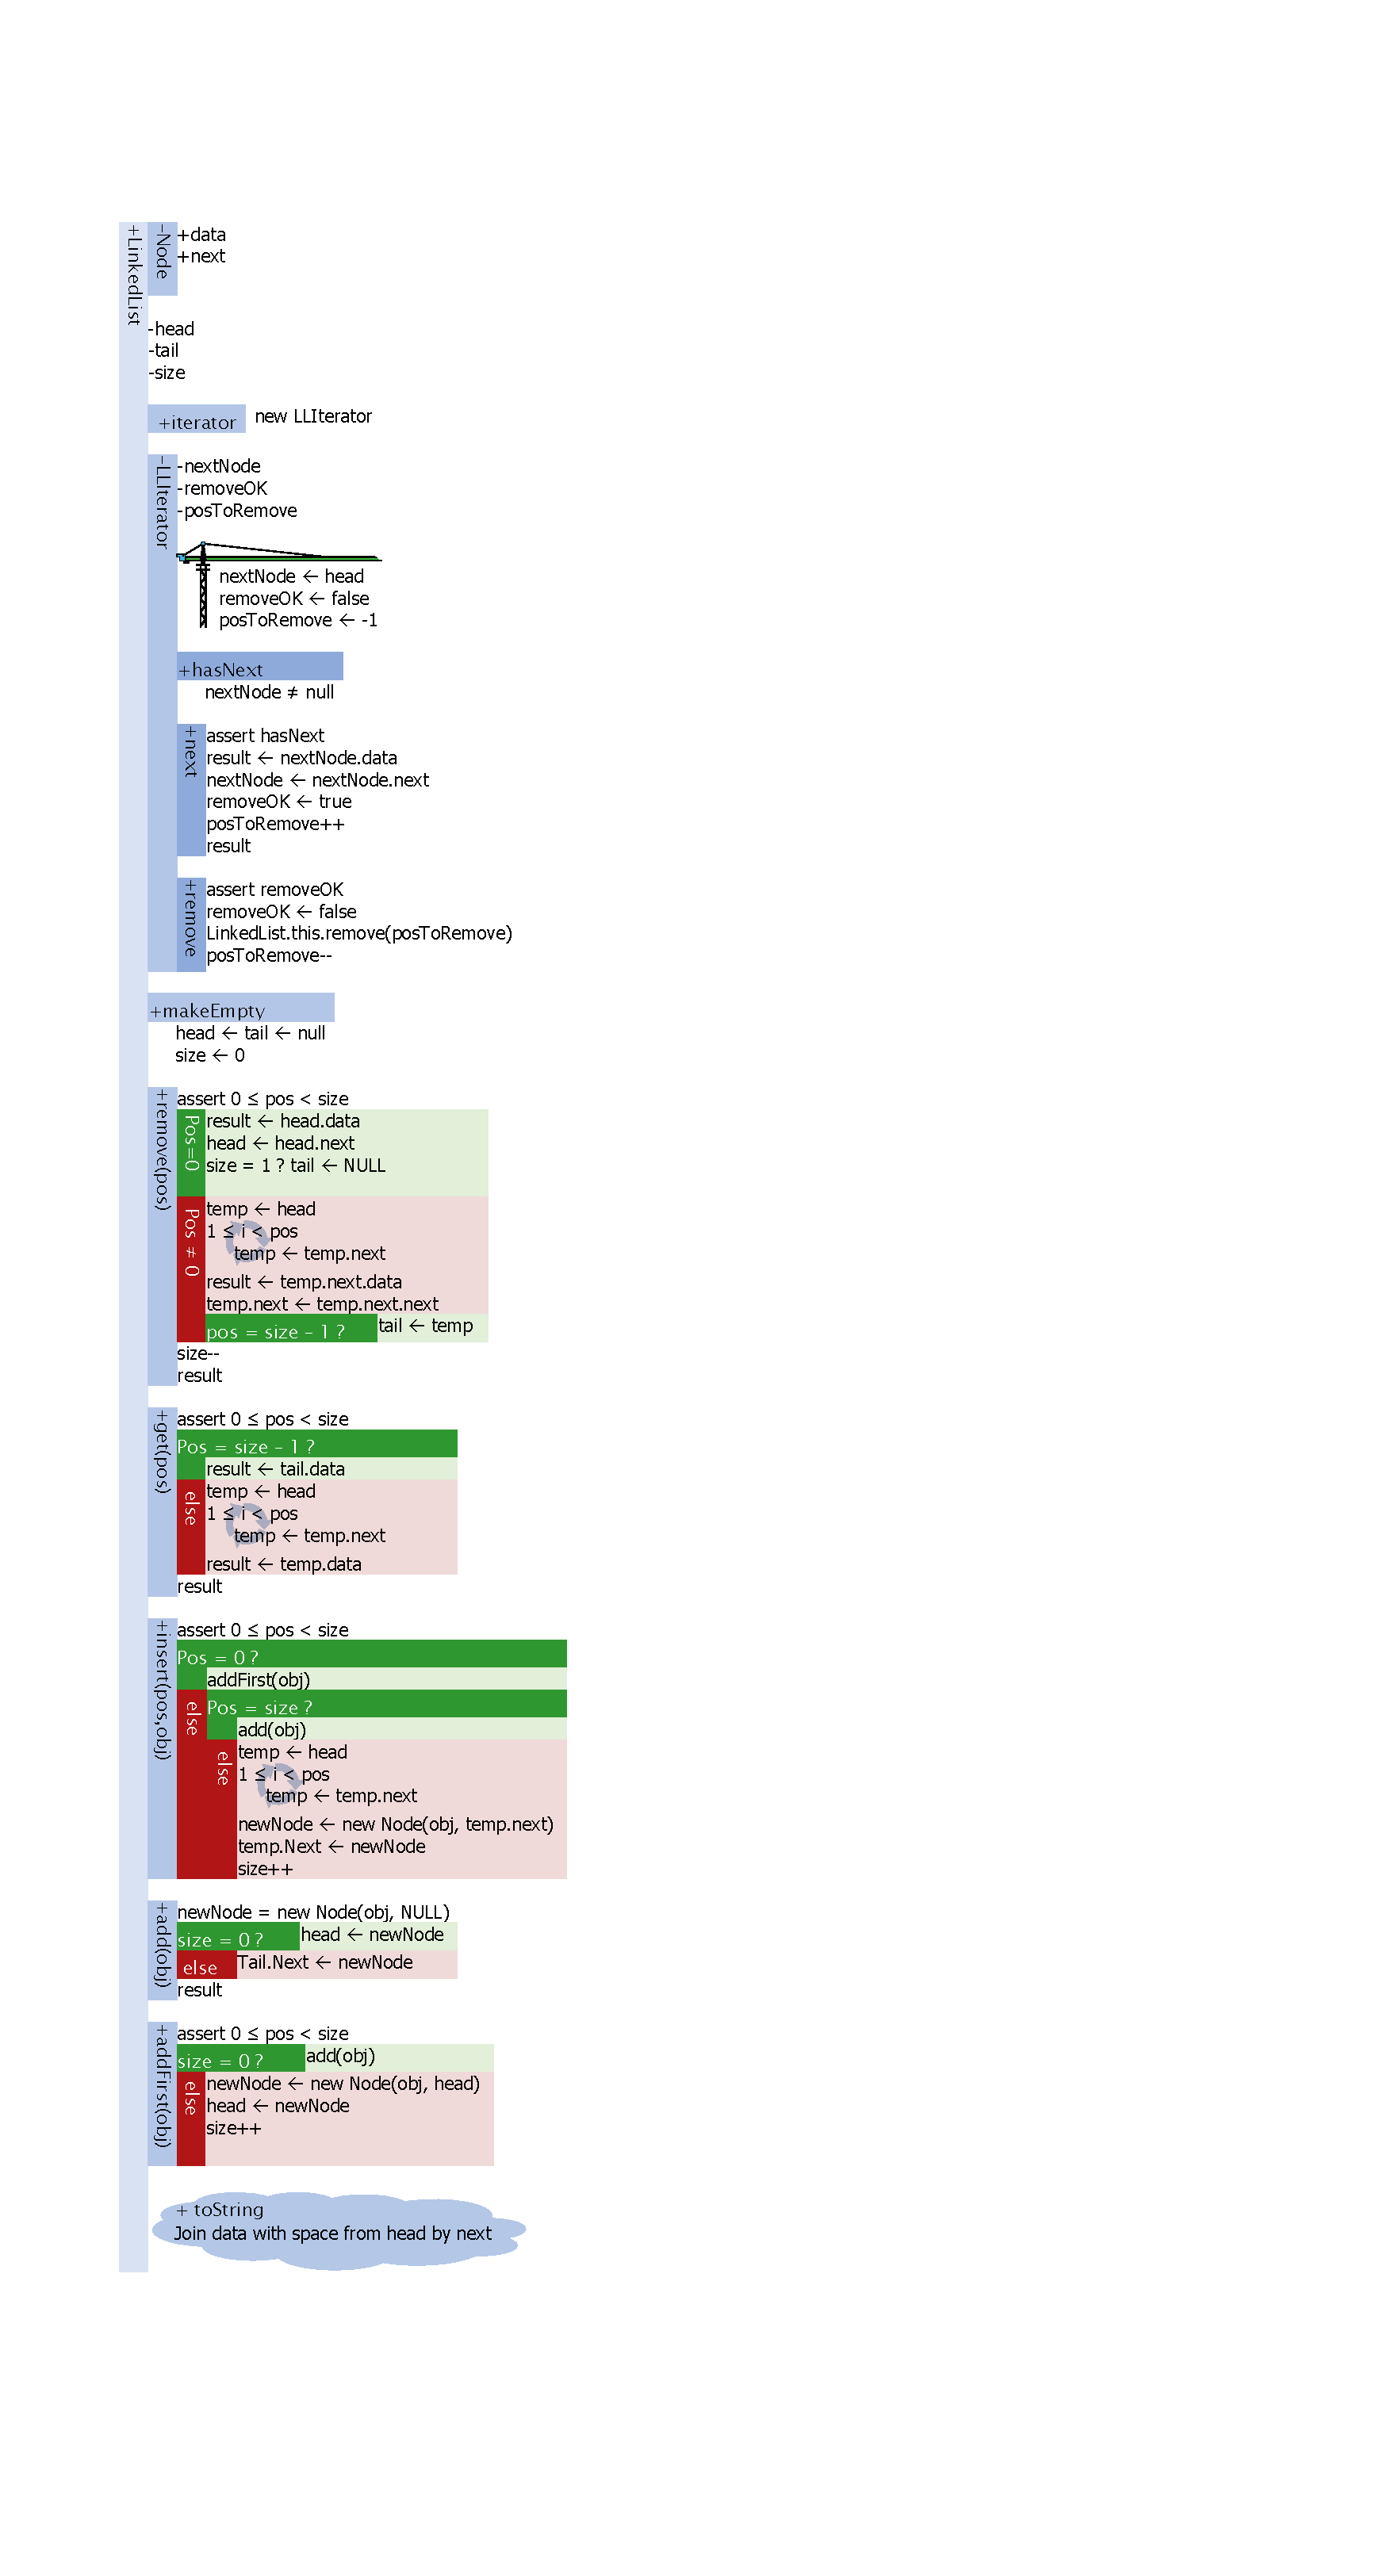
\includepdf[pages=-]{./files/Linked-List-Compact-Representation.pdf}